%%%%%%%%%%%%%%%%%%%%%%%%%%%%%%%%%%%%%%%%%%%%%%%%%%%%%%%%%%%%%%%%%%%%%%%%%%%%%%%%%%%%%%%%%
% Section 7: Routing in RS2
%	This section contains a description of the following:
%	- Wires and connection types in RS2 (wire connections, routethroughs, etc.)
%	- How to route nets in RS2 using RouteTrees
%	- Three-part routing structure for nets.
%	- Vivado ROUTE strings and intrasite routing.
%%%%%%%%%%%%%%%%%%%%%%%%%%%%%%%%%%%%%%%%%%%%%%%%%%%%%%%%%%%%%%%%%%%%%%%%%%%%%%%%%%%%%%%%%
\newpage
\section{Routing} \label{sec:routing}
After placement, all \cells of a design have been mapped to \bels, and their
corresponding \cellpins mapped to \belpins. The next (and final) step of the
FPGA implementation flow is to physically wire together the used \belpins. This
is known as routing. Routing involves taking each logical \net of a design,
determining the \belpins they are connected to (based on the \cellpins), and
finding a list of physical wires that electrically connect the pins together.
This section details how routing is done in RS2.

\subsection{Wires and Wire Connections} \label{wireConnSection}
Routing in RS2 is done using \cls{Wire} objects, which are described in
\autoref{wireSection}. \cls{Wire}s are uniquely identified by their
corresponding tile and wire name (i.e. tileName/wireName), and are connected
through \cls{Connection} objects. There are two types of wire connections:

\begin {enumerate}
  \item \textbf{PIP Connections}: Connect two different wires through a
  Programmable Interconnect Point. Most PIP connections are found in
  switchbox tiles of an FPGA part (as shown in \autoref{fig:switchboxPIP}).
  These types of connections are important to FPGA routing, because they
  dynamically configure the routing network for a given design.
   
  \item \textbf{Non-PIP Connections}: Connect the same physical wire across two
  different tiles. In general, wires stretch across multiple tiles in a device, having
  a different name in each tile. This is demonstrated in
  \autoref{fig:wireFigure}. The example wire shown in the figure spans 5
  different tiles, but has a different name in each. To save space, only the
  source and sink wire segments are kept in RS2 data structures
  (i.e. \texttt{INT\_X1Y1/E2BEG4}, \texttt{INT\_X2Y1/E2MID4}, and
  \texttt{INT\_X3Y1/E2END4}). The source segment is connected to each sink
  segment through a non-PIP wire connection. It is also possible to have non-PIP
  connections within a \tile, but this is rare.
\end{enumerate} 

\begin{figure}[H]
\centering
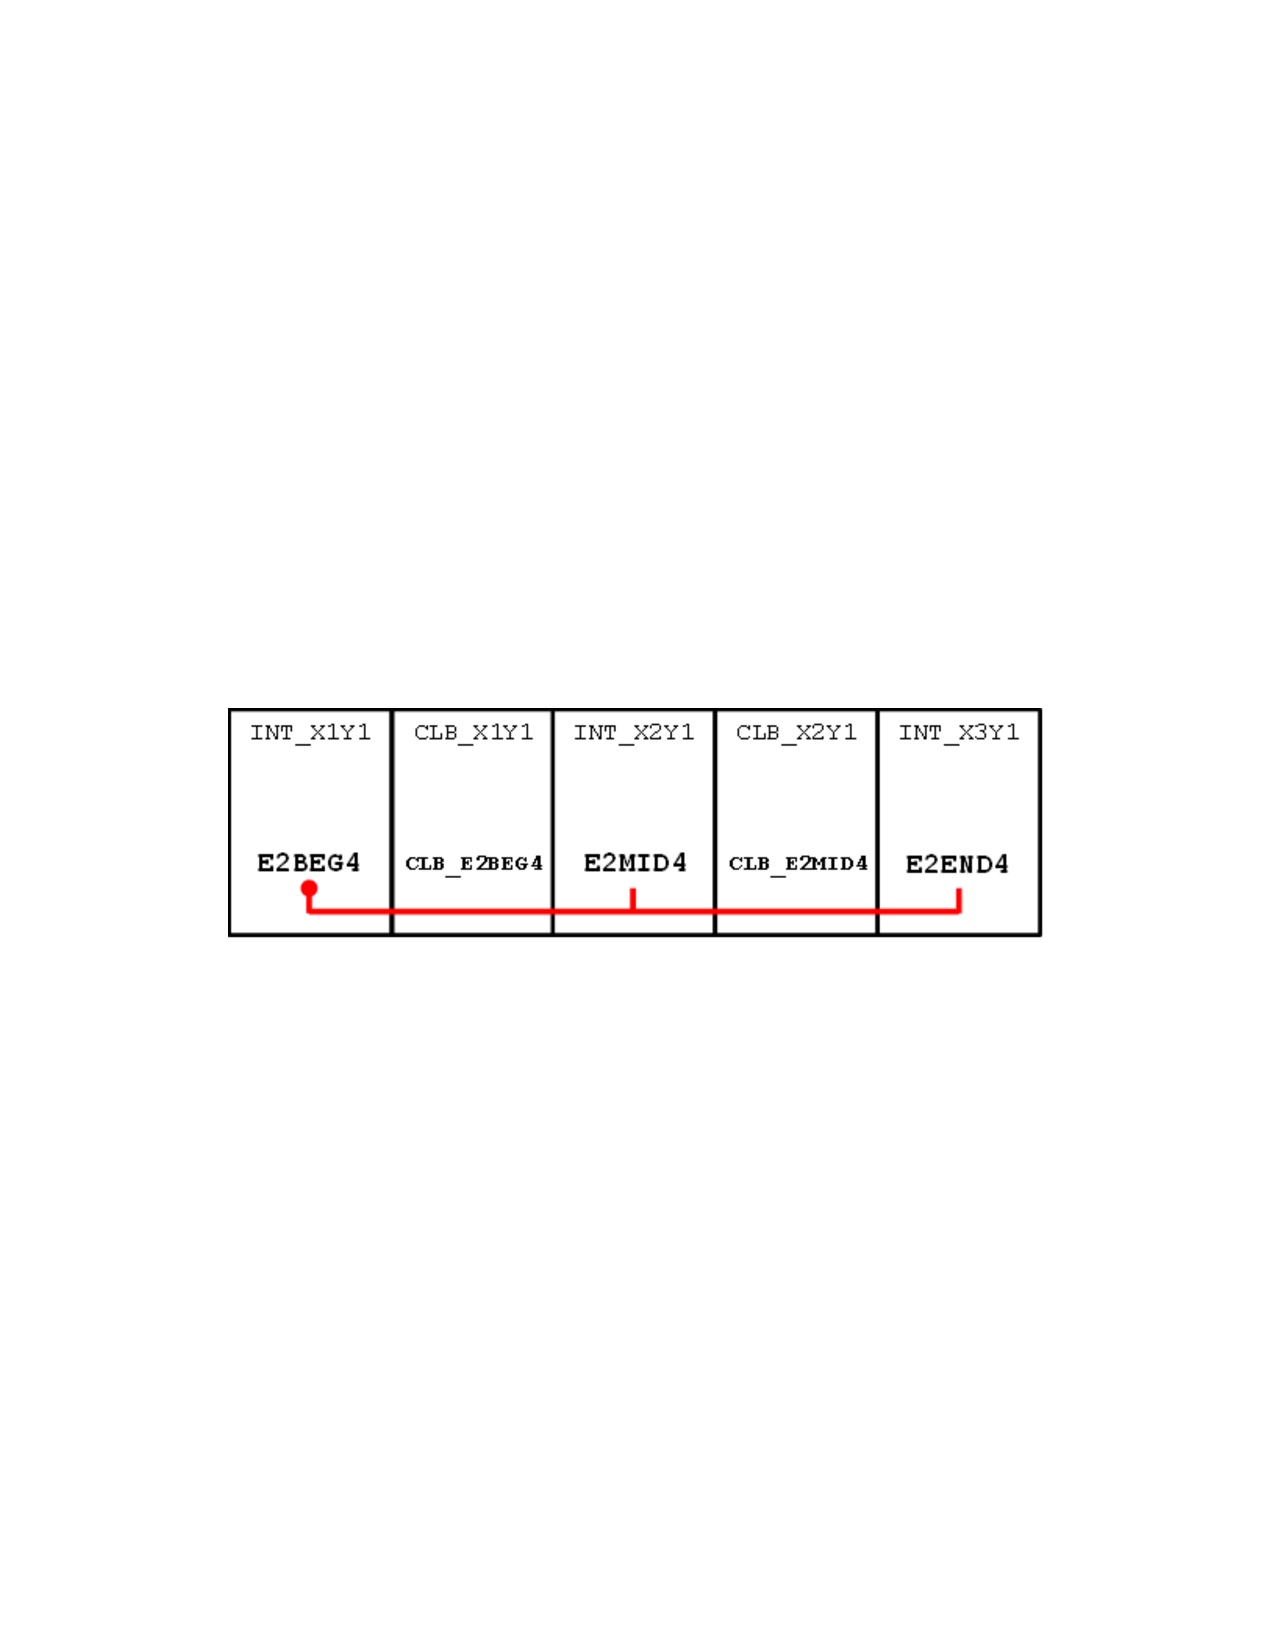
\includegraphics[width=0.8\columnwidth]{wireFigure}
\caption{A wire in an FPGA illustrating how each part of the wire has a
different name depending on the tile it is located in}
\label{fig:wireFigure}
\end{figure}

\subsection{Traversing Wire Objects}
Traversing through wires in a device is straightforward. Given a handle to a
\cls{Wire} object named "mywire" or a \cls{Connection} object named
"conn", the following function calls can be used:

\begin {itemize}
  \item \texttt{mywire.getWireConnections()}: Returns a collection of all
  \cls{Connection} objects whose source is ``mywire''. This collection can
  be iterated over to find all places a specific wire goes (i.e. what wires it
  connects to).
  \item  \texttt{conn.isPip()}: Returns true if the wire connection ``conn'' is
  a PIP connection. Returns false otherwise.
  \item \texttt{conn.getSinkWire()}: Returns the sink wire of a wire connection.
\end{itemize} 

\noindent
In general, these are the only three functions that are needed to
search through the wires of a FPGA device. It is important to note however that
the first wire in the route has to be either (a) created using a \cls{TileWire}
constructor, or (b) retrieved from a function call of another object (such as
\texttt{SitePin::getExternalWire()}). \autoref{code:connections} demonstrates
how to iterate over \cls{Connection} objects. To gain a better
understanding of how to use \cls{Wire}s and \cls{Connection}s, see the
\pgm{HandRouter} example in the RS2 repository.

\subsection{Other Types of Connections} \label{otherConns}
Along with PIP and non-PIP wire connections, there are several other types of
connections in RS2. The source of the connection is always a \cls{Wire}
object, but the sink object differs. A description of these connections is found
below:

\begin {itemize}
  
  \item \pgm{Site Pin Connections}: Connects a \cls{Wire} to a \cls{SitePin}.
  The function call \texttt{conn.get\-SitePin()} can be used to get the sink
  \cls {SitePin} object.
  \item \pgm{Terminal Connections}: Connects a \cls{Wire} to a \cls{BelPin}. The
  function call \texttt{conn.get\-BelPin()} can be used to get the sink \cls
  {BelPin} object.
  \item \pgm{Site Routethrough Connections}: Connects an input site \cls{Wire}
  to an output site \cls{Wire}. A \cls{Site} in Vivado can be configured to pass
  the signal on an input \cls{SitePin} directly to an output \cls{SitePin}.
  These connections are represented as routethroughs in RS2 and can be
  determined with the function call \texttt{conn.isRoutethrough()}.
  \pgm{NOTE}: Before using this type of connection when building a
  routing data structure, make sure the \cls{Site} is unused.
  \item \pgm{BEL Routethrough Connections}: Connects an input BEL \cls{Wire} to
  an output BEL \cls{Wire}. Similarly to a \cls{Site} routethrough, LUTs in
  Vivado can also be configured as routethroughs. In this case, the signal on one of the
  input pins of the LUT is passed directly to the output pin of the LUT. A BEL
  routethrough connection can be used to configure a LUT as a routethrough in
  RS2.
  \pgm{NOTE}: Before using this type of connection, make sure the LUT is
  unused (i.e. no cell is placed on it).
\end{itemize}

\noindent
When traversing through the device data structure, a generic \cls{Connection}
object is usually used. This connection can refer to any of the connections
described so far in this documentation. \autoref{code:connections} demonstrates
how to iterate through different \cls{Connection} types in RS2.

\begin{lstlisting}[caption=How to iterate over Connections in RS2,
label=code:connections] 
// Get a handle to a wire
Wire wire = sitePin.getExternalWire();

// Iterate over all WireConnections
for (Connection conn : wire.getWireConnections()) {
	Wire sinkWire = conn.getSinkWire();

	if (conn.isPip()) {
		// Do something with a PIP
	} 
	else if (conn.isRoutethrough()) {
		// Do something with a routethrough
	} 
	else {	
		// Do something with a regular wire connection				
	}
}

// Iterate over all Pin Connections
for (Connection conn : wire.getPinConnections() ) {
	SitePin pin = conn.getSitePin();
	// Do something with the SitePin
}

// Iterate over all Terminal Connections
for (Connection conn : wire.getTerminals()) {
	BelPin bp = conn.getBelPin();
	// Do something with the BelPin
}

// Iterate over all connections at the same time
Iterator<Connection> connIt = wire.getAllConnections().iterator();

while (connIt.hasNext()) {
	Connection conn = connIt.next();
	
	if (conn.isPinConnection()) {
		//do something with the site pin
	}
	else if (conn.isTerminal()) {
		//do something with the bel pin 
	}
	else if (conn.isPip()) {
		//do something with the pip wire connection
	}
	else {
		//do something with regular wire connection.
	}
}
\end{lstlisting}

\subsection{RouteTrees}

\cls{Wire}s and \cls{WireConnection}s are the fundamental objects used to
specify and explore routing in RS2, but they need to be organized in
a higher-level data structure to give meaning to the route of a \cls{CellNet}.
In the original RapidSmith, creating this data structure was up to the user.
RS2 introduces the \cls{RouteTree}, which can be see in
\autoref{fig:routeTreeDS}.

\begin{figure}[H]
\centering
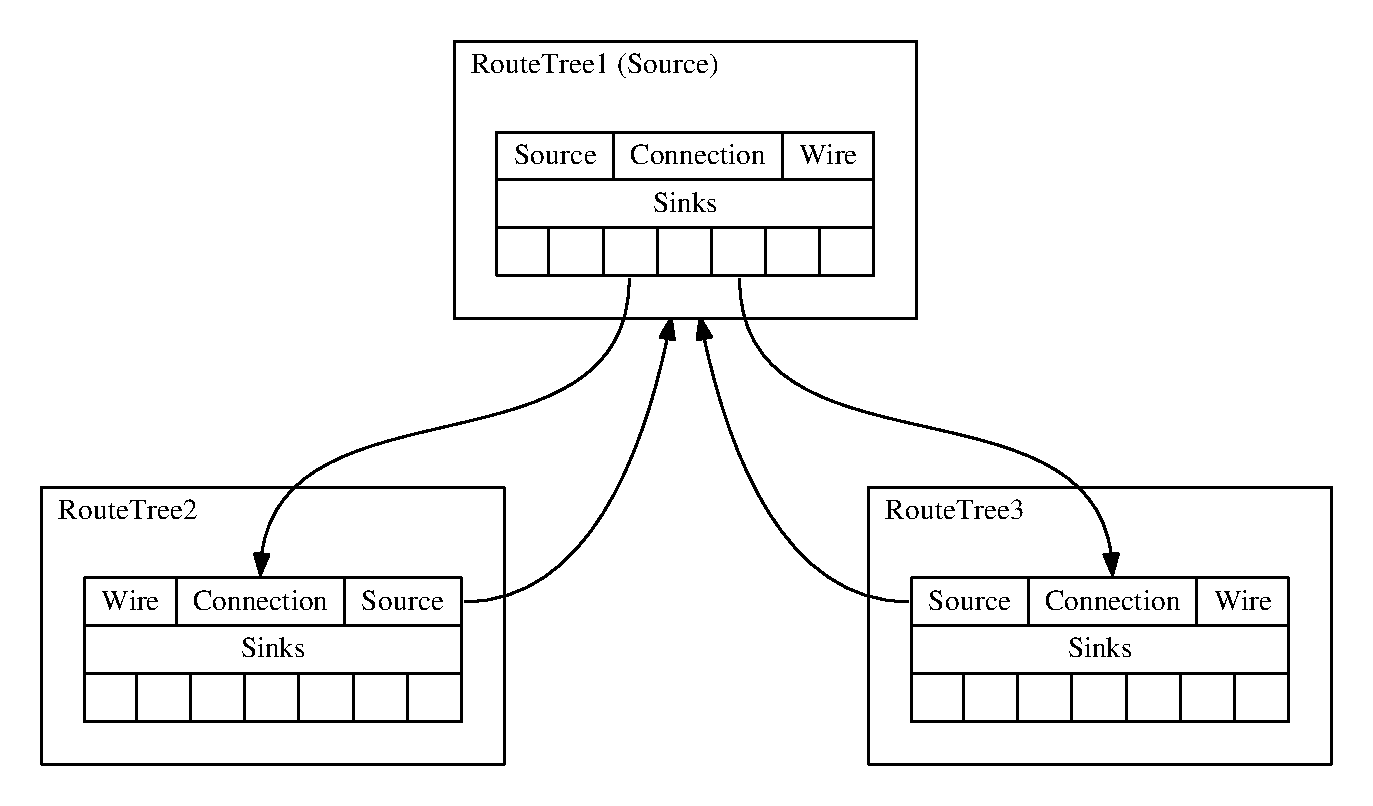
\includegraphics[width=0.8\columnwidth]{routeTreeDS.eps}
\caption{Visual representation of the \cls{RouteTree} data structure.}
\label{fig:routeTreeDS}
\end{figure}

\noindent
As the figure shows, a \cls{RouteTree} is a simple tree data structure. Each
node in the tree represents a physical wire, and is connected to other nodes
(wires). Edges in the tree represent wire connections (i.e. how one wire
connects to another). A \cls{RouteTree} can also be conceptually thought of as
a graph, with a single ``starting'' node and several ``sink'' nodes. A
\cls{RouteTree} node contains the following members:

\begin{itemize}
  \item \pgm{Wire}: The physical \cls{Wire} object that the \cls{RouteTree} node
  represents. This can be either a \cls{TileWire} or \cls{SiteWire}.
  \item \pgm{Source}: A link to the the parent \cls{RouteTree} node 
  \item \pgm{Connection}: The \cls{Connection} taken from the \pgm{parent}
  RouteTree node to reach the \pgm{current} RouteTree node. In other words, it
  is the \cls{WireConnection} object that was taken from the parent wire to reach the current wire.
  \item \pgm{Sinks}: A list of child nodes. There is no limit
  to how many children a \cls{RouteTree} node can have.
  \item \pgm{Cost} (not shown): An optional cost field for routers 
\end{itemize}

\noindent
A complete \cls{RouteTree} specifies how the source of a
\cellnet is physically connected to all of its sinks. \autoref{fig:routeTree}
shows an example of a complete \cls{RouteTree} in RS2. 

\begin{figure}[H]
\centering
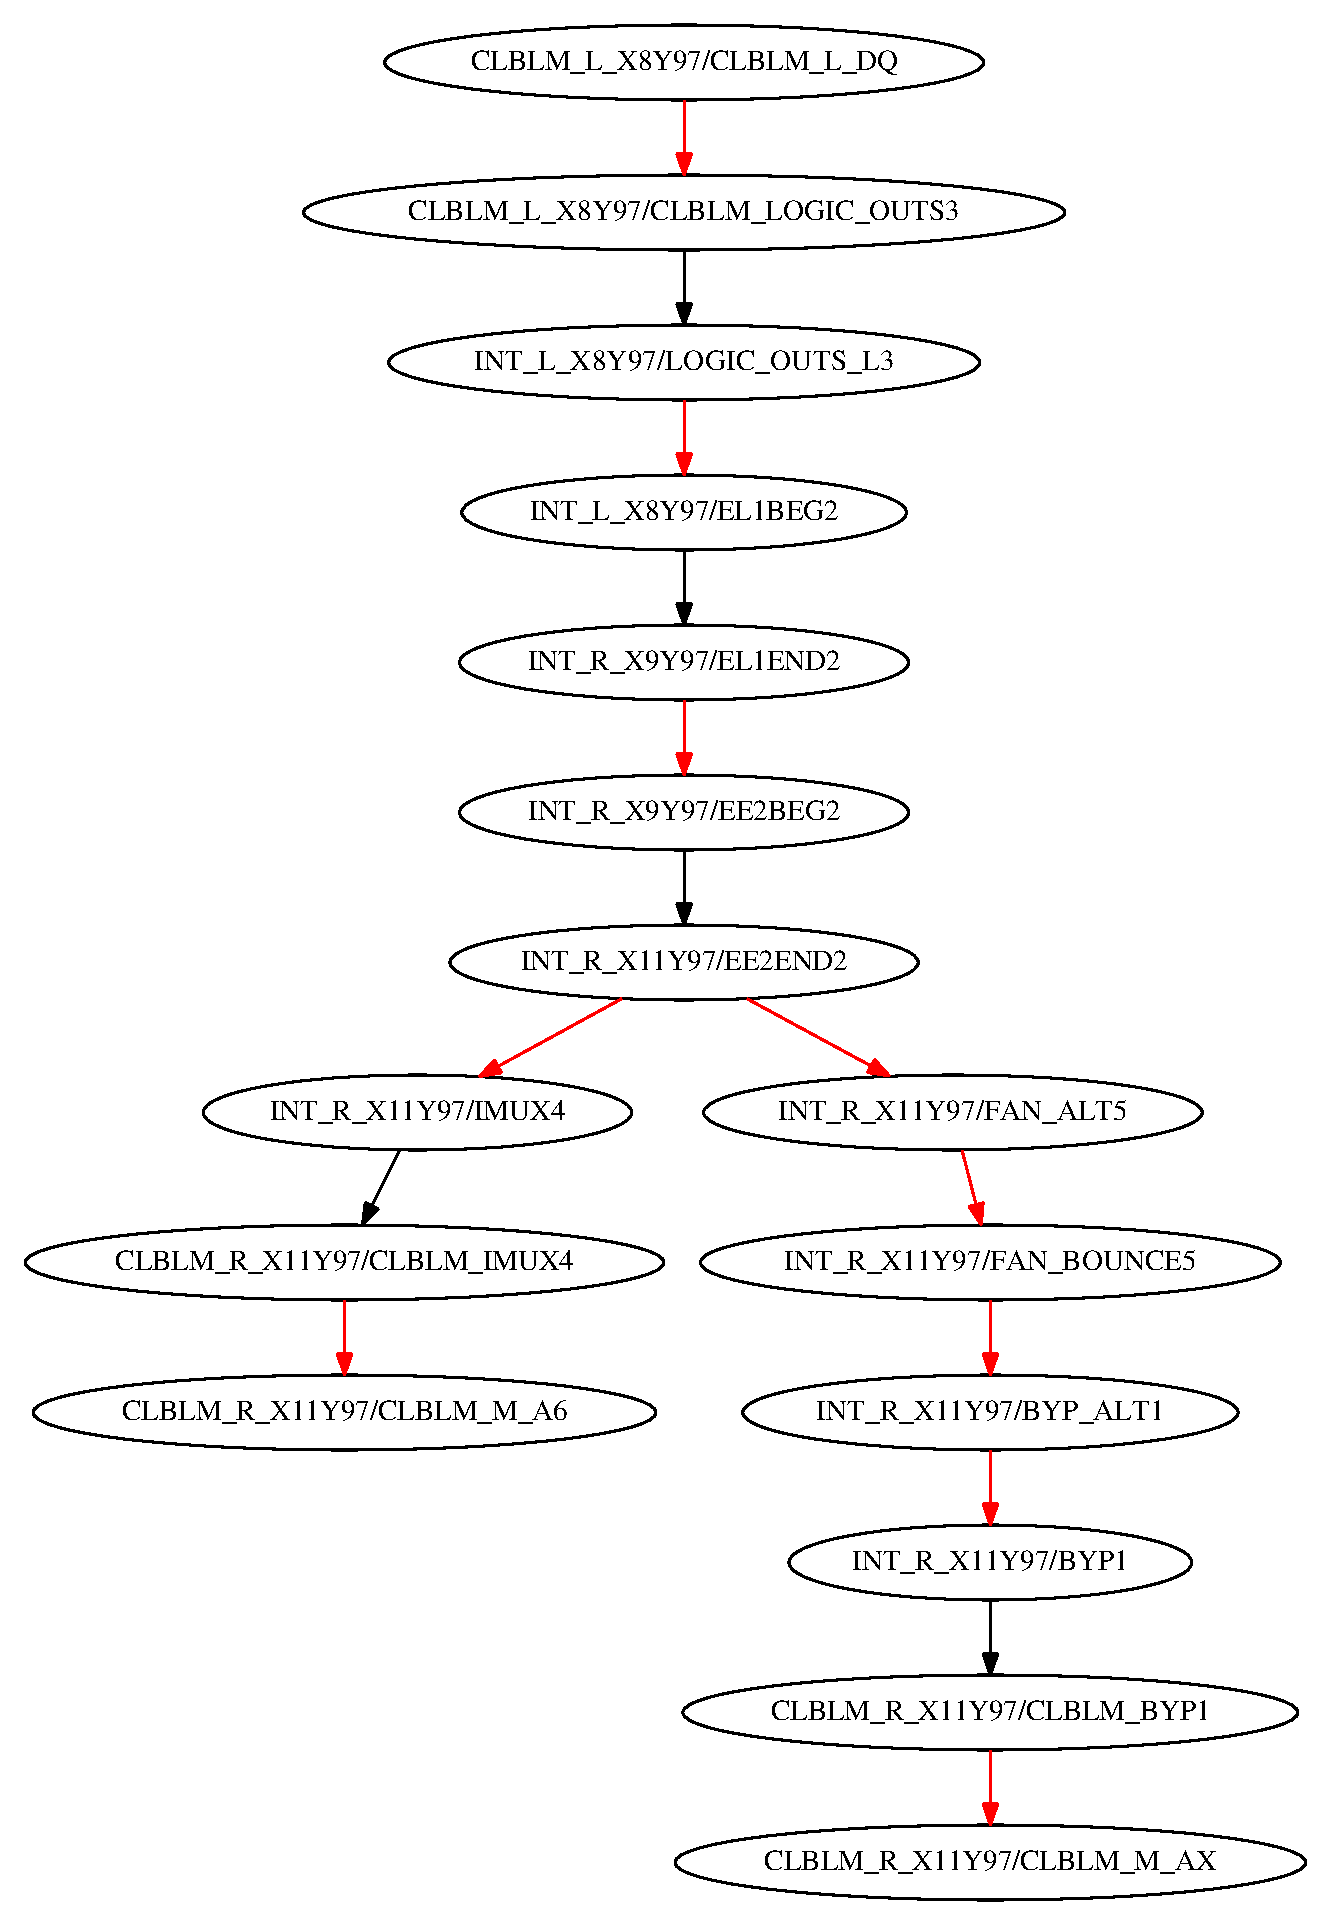
\includegraphics[width=0.65\columnwidth]{routeTree.eps}
\caption{A visual representation of a RS2 RouteTree. Nodes represent
\cls{Wire}s, red edges represent \cls{PIP} wire connections, and black edges
represent non-PIP wire connections. This specific RouteTree was created from
the \pgm{AStarRouter} example.}
\label{fig:routeTree}
\end{figure}

\noindent
In this case, the \cellnet that is being routed has once source pin, and two
sink pins. The source pin is connected to wire ``CLBLM\_L\_X8Y97/CLBLM\_L\_DQ'',
and the sink pins are connected to the wires ``CLBLM\_R\_X1Y97/CLBLM\-\_M\_A6''
and ``CLBLM\-\_R\_X11Y97/CLBLM\_M\_AX''. Starting from the source, wires are
traversed downward (via wire connections) until the target wires are reached.
\autoref{code:routeTree} demonstrates the basic usage of \cls{RouteTree}s in
RS2. The \pgm{DesignAnalyzer}, \pgm{AStarRouter}, and \pgm{HandRouter}
examples described in \autoref{examples} also demonstrate how to traverse and
build a \cls{RouteTree}.

\begin{lstlisting}[caption=Building a RouteTree,
label=code:routeTree] 
// Find a Wire to start the RouteTree at
Site site = device.getSite("SLICE_X5Y84");
SitePin pin = site.getSitePin("DQ");
Wire startWire = sink.getExternalWire();

// Create the first node in the RouteTree 
Queue<RouteTree> rtQueue = new LinkedList<RouteTree>();
RouteTree start = new RouteTree(startWire);
rtQueue.add(start);

// Build up the RouteTree somehow 
while (!amDone()) {
	RouteTree current = rtQueue.poll();
	Wire wire = route.getWire();

	for (Connection conn : wire.getWireConnections()) {
		// add qualified connections to the RouteTree
		if (isQualified(wire)) {
			RouteTree tmp = current.addConnection(conn);
			rtQueue.add(tmp);
		}
	}
}

\end{lstlisting}

When a design is imported from Vivado, the routing information is parsed and
loaded into \cls{Route\-Tree}s for each \cellnet. On design export, the
\cls{RouteTree} for each \cls{CellNet} is traversed and converted into a Vivado
ROUTE string. A user can use custom data structures to route a design, but it
needs to be \pgm{converted to an equivalent RouteTree data structure} before
exporting the design to Vivado.  

\subsection{Three Part Routing}
In RS2, there are three sections to a routed  \cellnet. 

\begin{enumerate}
  \item The portion of the net that starts at the source \belpin, and is routed
  to an output \sitepin. This part of the route exists completely inside of
  \site boundaries.
  \item The portion of the net that starts at the output \sitepin of part (1),
  and is routed to several sink \sitepins. This part of the route is
  called the ``INTERSITE'' route because it connects \sites together. A typical
  router is responsible for routing this section of the net\footnote{VCC and
  GND nets don't follow this pattern. The only difference for VCC and GND is
  that they can have multiple intersite nets.}.
  \item The portion of the net that start at an input \sitepin from part (2),
  and is routed to a sink \belpin. Since there can be several sink pins in a
  \cellnet, this section of the net can have more than one component. This part
  of the route also exists completely inside of \site boundaries. 
\end{enumerate}

\noindent \autoref{fig:threePartRouting} shows an example of the three parts of
a routed \cellnet.

\begin{figure}[H]
\centering
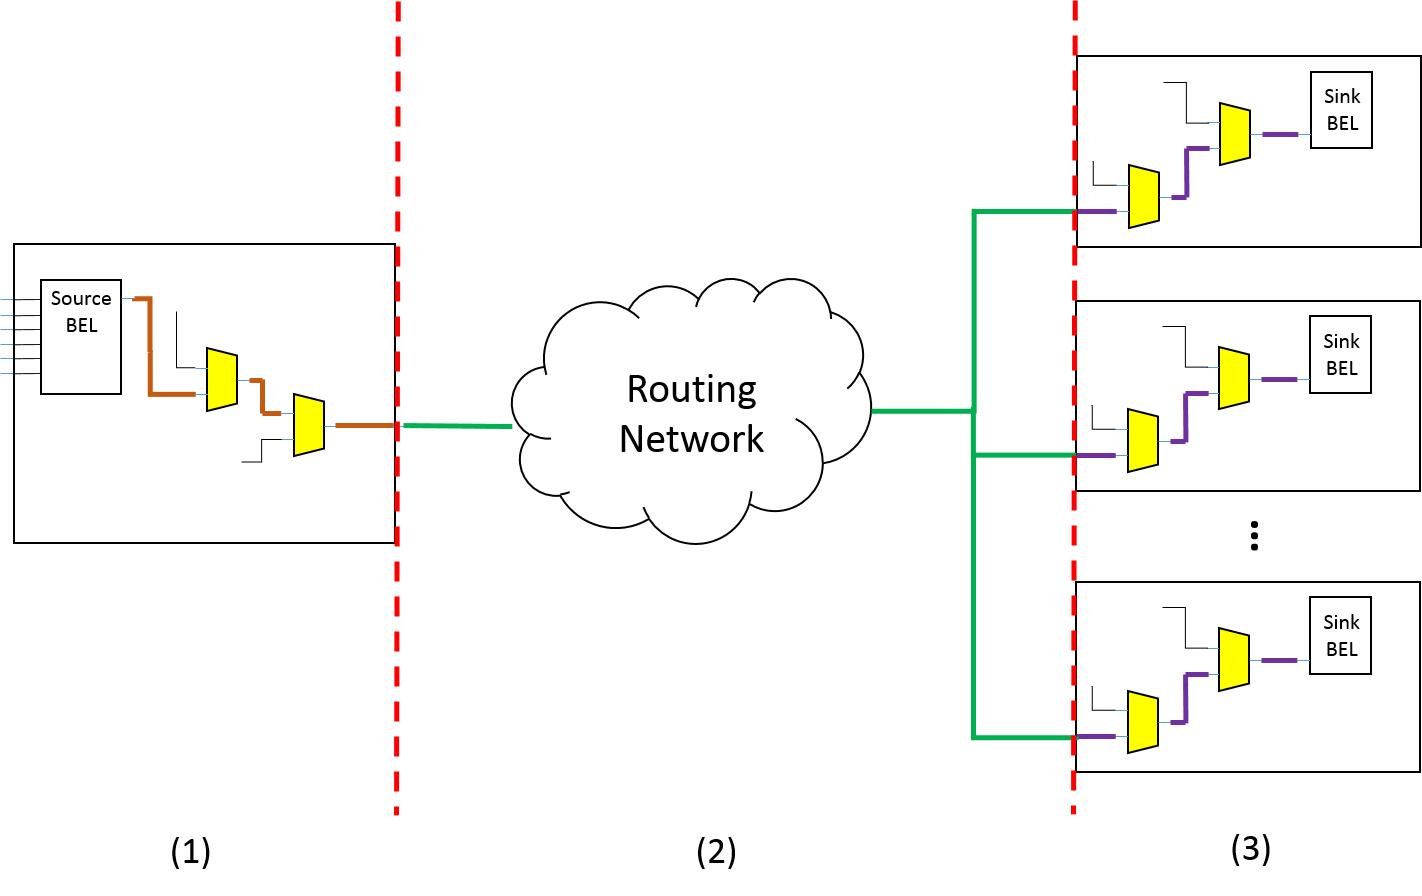
\includegraphics[width=1\columnwidth]{threePartRouting.png}
\caption{The three sections of a RS2 route.}
\label{fig:threePartRouting}
\end{figure}

\noindent 
There is a \routeTree object associated with each section of the
three-part routing. A source \routeTree represents the orange wires in the
figure above (part 1). An intersite \routeTree represents the green wires in the
figure above (part 2). A list of sink \routeTrees represents the purple
wires in the figure above (part 3, with a different \routeTree object for each
\site). It is important to note that INTRASITE nets only have a source
\routeTree because they are completely contained within a \site.
\autoref{code:threePartRouting} demonstrates how to utilize three part routing
in RS2. When a design is imported into RS2, the routing sections
of each \cellnet are created automatically.

\begin{lstlisting}[caption=Three-part routing in RS2,
label=code:threePartRouting]
// Get a handle to a routed net in the design 
CellNet net = design.getNet("myNet");

// Handling the source RouteTree
RouteTree source = net.getSourceRouteTree();
net.setSourceRouteTree(createSourceRoute());

// Handling the intersite RouteTree
RouteTree intersite = net.getIntersiteRouteTree();
net.addIntersiteRouteTree(createIntersiteRoute());

// Iterate over a list of sink RouteTrees
for (RouteTree rt : net.getSinkSitePinRouteTrees()) {
	// do something with the RouteTree
}

// Or, get a RouteTree based on a SitePin
for(SitePin sitePin : net.getSitePins()) {
	if (sitePin.isInput()) {
		RouteTree sinkTree = net.getSinkTree(sitePin);
		// do something with the RouteTree
	}
}

// Add a new sink RouteTree that starts at a SitePin

net.addSinkRouteTree(sitePin, createSinkRouteTree(sp));
\end{lstlisting}

\subsection{Routing in Vivado}
The reason a three-part routing distinction is necessary in RS2, is due
to how routing is represented in Vivado. Inside \site boundaries, a route is
represented using \site \pips. A string of enabled \pips determines what pins
are connected together within the \site. Between \site boundaries, a route is
instead represented using wires. The wires are formatted into a Vivado ROUTE
string, which uniquely specifies the intersite route for a net. The three-part
routing representation makes this distinction explicit to the users of
RS2 (it also makes import/export easier). When a design is exported from
Vivado, the intrasite portions of a net are exported as \site \pips, and the
intersite portion of the net is exported as wires.

\begin{lstlisting}[numbers=none, keywordstyle=, stringstyle=]
% An example of a string of used site pips in Vivado
{IUSED:0 IBUFDISABLE_SEL:GND INTERMDISABLE_SEL:GND}

% An example of a Vivado ROUTE string
 { CLBLL_LL_AQ CLBLL_LOGIC_OUTS4  { NW6BEG0 NE2BEG0 WR1BEG1 IMUX_L34
IOI_OLOGIC0_D1 LIOI_OLOGIC0_OQ LIOI_O0 }  IMUX_L1 CLBLL_LL_A3 }  
\end{lstlisting}

\subsection{IntrasiteRouting}
On design import, the \site \pip information extracted from Vivado is stored
into RS2 data structures, and used to resconstruct the three-part
routing view. This gives the user two options when dealing with intrasite
routing in RS2: (1) use the three-part routing data structures, or (2)
use the set of enabled \site \pips that exist in each \site. It is up to user
preference for which representation to use when writing a CAD tool, but in
order to export a design back into Vivado the three-part routing data
structures need to be converted to \site \pips and assigned to their
corresponding \site. \autoref{code:sitePips} demonstrates how this is
currently done. This step needs to be taken \pgm{only when you have modified the
intrasite routing} for a \site. We are working on improving the API for \site
\pips, and creating a way to automate conversion from three-part routing to
\site \pip information.

\begin{lstlisting}[caption=Configuring Site Pips,
label=code:sitePips]
// Get a handle to a Design and a Site
CellDesign design = vcp.getDesign();
Device device = vcp.getDevice();
Site site = device.getSite("SLICE_X5Y84");

// Get a list of used site wires somehow (this is up to you)
Set<Wire> usedSiteWires = getUsedWires(site);

// Convert the list of wires to their integer enumeration
Set<Integer> usedPipWires = usedSiteWires.stream()
										 .map(w -> w.getWireEnum())
										 .collect(Collectors.toSet());

// Set the used site pips with the design class
design.setUsedSitePipsAtSite(site, usedPipWires);

\end{lstlisting}
